\documentclass[a4paper, amsfonts, amssymb, amsmath, reprint, showkeys, nofootinbib, twoside]{revtex4-1}
\usepackage[english]{babel}
\usepackage[utf8]{inputenc}
\usepackage[colorinlistoftodos, color=green!40, prependcaption]{todonotes}
\usepackage[pdftex, pdftitle={Article}, pdfauthor={Author}]{hyperref}
\usepackage{amsthm}
\usepackage{mathtools}
\usepackage{physics}
\usepackage{xcolor}
\usepackage{caption}
\usepackage{hyperref}
%\hypersetup{colorlinks=true, linkcolor=blue, urlcolor = blue}
\usepackage{amsmath}
\usepackage{amssymb}
\usepackage{graphicx}
\graphicspath{Images}
\usepackage[left=23mm,right=13mm,top=35mm,columnsep=15pt]{geometry} 
\usepackage{adjustbox}
\usepackage{placeins}
\usepackage[T1]{fontenc}
\usepackage{float}
%\usepackage{longtable}
\usepackage{csquotes}
\usepackage{refstyle}
\usepackage{lipsum}

\begin{document}

\title{Study of I-V Characteristics of Solar Cell}
\author{Swaroop Ramakant Avarsekar}
\email{swaroop.avarsekar@niser.ac.in}
\affiliation{School of Physical Sciences, National Institute of Science Education and Research, HBNI, Jatni -752050, India}
\date{\today}

\begin{abstract}
This experiment aims to study the V-I characteristics of the solar cell illuminated by sunlight and tubelight at different wavelengths and compare the power output in each case. The solar cell is a p-n junction diode where transfer of charge carriers across the junction takes place through photovoltaic effect. Various factors such as open circuit voltage, short circuit current, maximum power output are obtained. The V-I characteristics of solar cell is similar to that of a p-n junction diode but it is slightly shifted due to short circuit current. From the experiment it is seen that the maximum power is generated when no filters are applied on the solar cell when placed under sunlight, with efficiency of ($2.30\pm0.16$) \% which proves a good method to harness energy from the sun, whereas efficiency under tubelight with no filter is ($1.10\pm0.07$)$\times10^{-2}$ \%.
\end{abstract}
	
\keywords{Photovoltaic effect, Fill factor, Open circuit voltage, Short circuit current}
	
\maketitle

\section{Theory}
Solar cell is a p-n junction diode which converts light energy to electrical energy. The current is generated by absorption of photons creating electron hole pair, which has energy greater than the band gap of the material and then collecting these charge carriers at the other end of the p-n junction respectively. In solar cell, the n region is usually thinner than p region to generate large power output, as it is necessary to shine the light to the depletion layer. By exposing the n side towards the light, with the metal contacts at the attached at each ends, the electron flows and current is obtained. 

The open circuit voltage ($V_{oc}$) is maximum voltage obtained from solar cell when current is zero and short circuit current {$I_{sc}$} is the maximum current obtained when voltage between two terminals of solar cell is zero.  Fill factor (FF) is the ratio of maximum power to open circuit voltage times short circuit current as in equation (\ref{e1}) . It is a measure of largest curve which will fit in the V-I curve. The efficiency ($\eta$) is ratio of energy output from the solar cell to the energy from the sunlight as seen in equation (\ref{e2}). The intensity of light and the temperature of solar cells contribute to the efficiency. Increase in temperature leads to reduction of band gap. Hence, these all factors are responsible for the rating of the solar cells.

\begin{equation}\label{e1}
	FF=\frac{P_{max}}{V_{oc}.I_{sc}}
\end{equation}

\begin{equation}\label{e2}
	\eta=\frac{V_{oc}.I_{sc}.FF}{P_{in}}
\end{equation}

$P_{in}$ is the input power.

Diode law is given by the equation(\ref{e1})-
\begin{equation}\label{dl}
	I=I_o[e^{\frac{qV}{nKT}}-1]
\end{equation}

where $I$ is total current flowing through diode, $I_{o}$ is dark saturation current, diode leakage current in the zero light, $V$ is applied voltage, $q$ is electron charge, $K$ is Boltzmann constant, $T$ is absolute temperature, n is the ideality factor.

For the solar cell, the current is generated so there is a correction term to the diode law, hence changing the eqaution (\ref{dl}) to equation (\ref{sl}).

\begin{equation}\label{sl}
	I=I_o[e^{\frac{qV}{nKT}}-1]-I_{L}
\end{equation} 

where $I_{L}$ is the current generated from solar cell.

\begin{figure}[H]
	\centering
	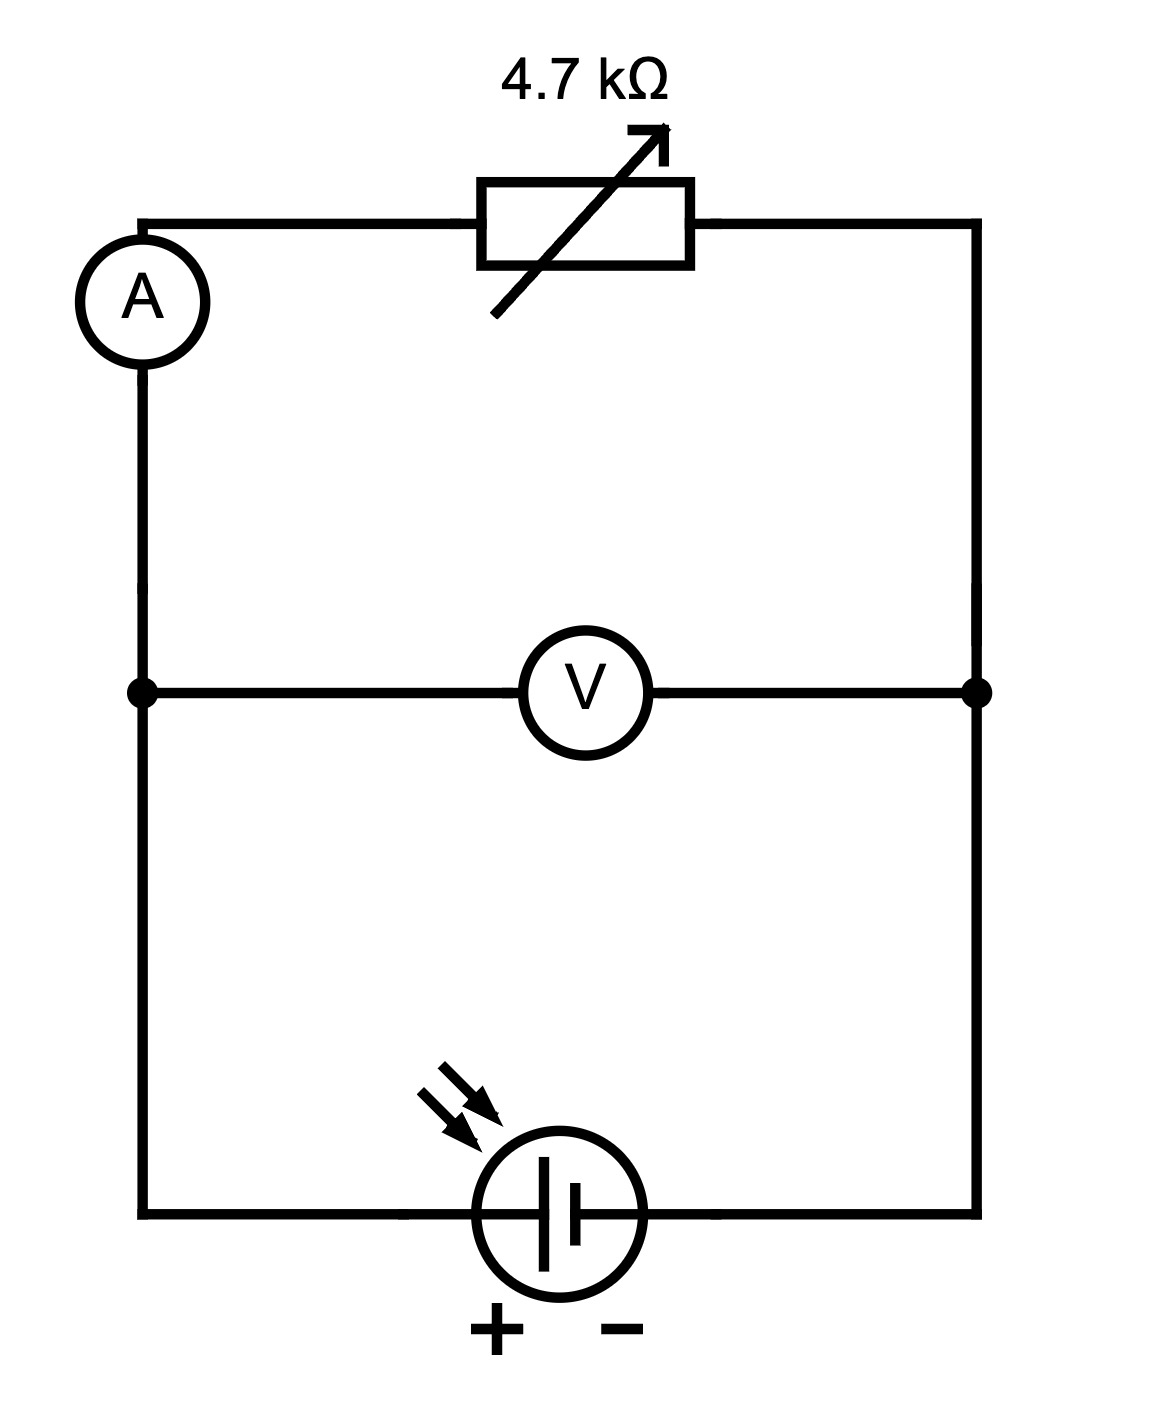
\includegraphics[scale=0.15]{1} 
	\caption{Circuit diagram for the I-V characteristics of solar cell.}
	\label{c}
\end{figure}

The V-I characteristics of solar cell is shown in figure (\ref{4}).

\begin{figure}[H]
	\centering
	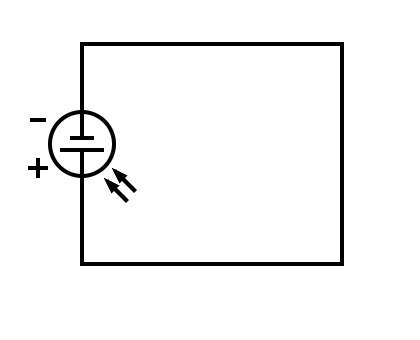
\includegraphics[scale=0.3]{3}
	\caption{Short circuit of solar cell}
	\label{sc}
\end{figure}

\begin{figure}[H]\label{vi}
	\centering
	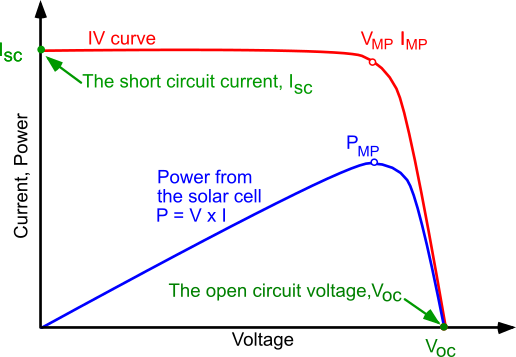
\includegraphics[scale=0.5]{4} 
	\caption{I-V characteristics of solar cell.}
	\label{4}
\end{figure}

\begin{figure}[H]
	\centering
	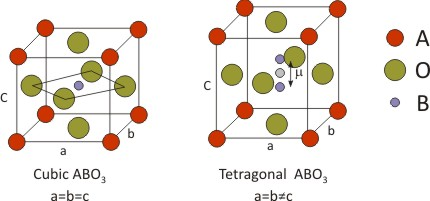
\includegraphics[scale=0.03]{2}
	\caption{Experimental setup}
	\label{e}
\end{figure}

\section{Experiment}
The voltage and current values are obtained from the solar cell under sunlight and tube-light from which power (P=V.I) was calculated. The V-I characteristics in both cases are shown in Figure (\ref{visun}) and (\ref{vitube}) and V-P curve is shown in Figure (\ref{vpsun}) and (\ref{vptube}).

\begin{figure}[H]
	\centering
	\includegraphics[width=\columnwidth,height=9cm]{5}
	\caption{V-I characteristics of solar cell under sunlight}
	\label{visun}
\end{figure}

\begin{figure}[H]
	\centering
	\includegraphics[width=\columnwidth,height=9cm]{7}
	\caption{V-P curve of solar cell under sunlight}
	\label{vpsun}
\end{figure}

\begin{figure}[H]
	\centering
	\includegraphics[width=\columnwidth,height=9cm]{6}
	\caption{V-I characteristics of solar cell under tube-light}
	\label{vitube}
\end{figure}

\begin{figure}[H]
	\centering
	\includegraphics[width=\columnwidth,height=9cm]{8}
	\caption{V-P curve of solar cell under tube-light}
	\label{vptube}
\end{figure}

\section{Calculation and Analysis}
The power is calculated from the formula P=V.I; The current is maximum for the case of no filter. The current is saturated upto a point and then decreases. The maximum current at low voltage is short circuit current ($I_{SC}$) and maximum voltage ($V_{OC}$) at low current is open circuit voltage. $I_{SC}$ and $V_{OC}$ for no filter, green yellow, pink, red are 102.4 mA and 6.13 V, 5.68 V and 47.5 mA, 57.8 mA and 5.91 V, 61.8 mA and 5.8 , 45.9 mA and 5.71 V, respectively for the case of solar cell under sunlight. The curves are higher for no filter, followed by pink, yellow, green, red. For the case of tube light the curves are higher for no filter, yellow, pink, red, green. 

The power is maximum with solar cell under sunlight in case of no filter with maximum output power as 349.65 mW.  157.42 mW for green filter, 221.76 mW for yellow filter, 233.772 mW for pink filter, 168.921 mW for red filter. The power linearly increases for each case , attains a peak and decreases. 

The fill factor can be calculated as shown in equation (\ref{e2}). The calculation for the case of solar cell in no filter under sunlight is shown below-
\begin{equation}
	FF=\frac{349.65}{102.4\times6.13}=0.557
\end{equation}

The size of solar cell is approximated to be 8.5 cm$\times$13 cm. With solar constant as 1370  $W/m^{2}$. We calculate $P_{in}$
\begin{equation}
	P_{in}=8.5 cm\times 13 cm*1370=15.1385 W
\end{equation}

\begin{equation}
	\eta_{sunlight}=\frac{P_{max}}{P_{in}}=\frac{349.65 mW}{15.1385 W}=0.0230  
\end{equation}

\begin{equation}
	\eta_{tubelight}=\frac{P_{max}}{P_{in}}=\frac{1.6642 mW}{15.1385 W}=0.00011
\end{equation}

The error in efficiency is calculated as follows:
\begin{equation}
\frac{\delta \eta}{ \eta}=\sqrt{\left( \frac{\delta V}{V}\right) ^{2}+\left( \frac{\delta I}{I}\right) ^{2}+\left( \frac{\delta L}{L}\right) ^{2}+\left( \frac{\delta B}{B}\right) ^{2}}
\end{equation}
where $\delta V$=0.01 V, $\delta I$=0.01 mA, $\delta L$=0.5 cm, $\delta B$= 0.5 cm which are least count of devices measuring voltage, current, length and breadth, respectively.
\begin{equation}
	\delta \eta_{sunlight}=0.0703\times0.023=0.0016
\end{equation}

\begin{equation}
	\delta \eta_{tubelight}=0.0703\times0.00011=7.73\times10^{-6}
\end{equation}

\section{Conclusion}
Solar cell is a p-n junction diode which converts light energy to electrical energy. Absorption of photons creating electron hole pair with the ends connected gives current. The solar cell was studied under sunlight and tube light with filters such as green, yellow, pink and red. The open circuit voltage ($V_{OC}$) is maximum voltage that could be obtained from solar cell and open circuit voltage ($I_{SC}$) is maximum current that could be drawn from the solar cell. The fill factor is the area of the largest curve which fits to V-I curve, defined as ratio of maximum power and product of $V_{OC}$ and $I_{SC}$. The open circuit voltage ($V_{OC}$) and short circuit current ($I_{SC}$) with solar cell under sunlight and tube light is 6.13 V,102.4 mA and 3.86 V, 0.76 mA, respectively. The efficiency of solar cell under sunlight and tubelight was found to be ($2.30\pm0.16$) \% and 
($1.10\pm0.07$)$\times10^{-2}$ \% respectively, implies that sunlight is excellent source to harness energy. 

The V-I characteristics under the aforementioned circumstances, the dependencies on the filters was not well distinguishable as it varied with sunlight and tube light. This may be caused due to error contributed as the temperature of solar cell was high after performing the experiment under sunlight. Several factors such as intensity of the light also comes into picture. The quality of the filter was not good. It could be improved as well. 


\section{References}
\begin{enumerate}
\item{\url{https://www.pveducation.org/}}
\item {\url{https://www.circuit-diagram.org}}
\item {\url{https://www.niser.ac.in/sps/sites/default/files/basic_page/p347_2023/7.IV_characeristics_Solarcell.pdf}}


\end{enumerate}

\end{document}